% =====================================================================
\section{Measurements to a target, bandwidth and sensitivity over a run}
\label{sm:speedup}
% =====================================================================

This section derives the number of measurements a sweep and an adaptive strategy need to reach a target
precision, from which the speedup of Eq.~\eqref{eq:speedup} and the bandwidth of Sec.~\ref{sec:sensitivity} of
the main text follow, and the course of the sensitivity over a run.

\paragraph{Sweep.} Where a sweep measures does not depend on what it has learned, so its expected information grows
at the constant rate $I_{\rm sweep}$ of Eq.~\eqref{eq:sweep-info} from its first measurement, and the van Trees bound
for the sweep is $\sigma\approx(\sigma_0^{-2}+nI_{\rm sweep})^{-1/2}$. This has the same $n^{-1/2}$ form as the refine
regime of an adaptive strategy; the two differ in the rate, $I_{\rm sweep}$ against $I_{\rm max}$. A single sweep
reaches this bound only once its posterior has one peak. Until the scan has passed over the dip it learns only that
the dip is not where it has looked, so its error, like that of an adaptive run, stays near $\sigma_0$ and then drops
when the dip is resolved, after about one pass of the window, or several at low SNR. What the sweep lacks is the
phase after that: an adaptive strategy moves its measurements onto the slope, so its rate rises from about
$I_{\rm sweep}$ to $I_{\rm max}$, while the sweep keeps spending a fraction of order $\Gamma/W$ of its measurements on
the line and stays at $I_{\rm sweep}$. Averaged over many passes the steps of the individual runs are smoothed out,
and the error follows the bound with no plateau and no cliff, as observed by \citet{dushenko2020sbed}.

\paragraph{Measurements to a target.} This too is a model of the error, so the window enters through its inverse
variance. An adaptive strategy pays the search cost $n_d$ of the elimination model first and then gains
$I_{\rm max}$ per measurement. Let $\sigma_{\rm tgt}$ (Hz) be the target precision, the standard deviation of $f_-$ at
which a run is considered done. The number of measurements to reach it is
\begin{equation}
  \begin{aligned}
  N_{\rm sweep}(\sigma_{\rm tgt})&=\frac{\sigma_{\rm tgt}^{-2}-\sigma_0^{-2}}{I_{\rm sweep}},\\
  N_{\rm ad}(\sigma_{\rm tgt})&=n_d+\frac{\sigma_{\rm tgt}^{-2}-12/\Delta d^2}{I_{\rm max}},
  \end{aligned}
  \label{eq:n-to-target}
\end{equation}
where the adaptive count follows the elimination model, Eqs.~\eqref{eq:elimination}--\eqref{eq:after-detection}:
$n_d$ measurements to detect the dip, after which the information starts at $12/\Delta d^2$ and grows by
$I_{\rm max}$ per measurement until it reaches $\sigma_{\rm tgt}^{-2}$. The sweep count uses the averaged rate, so it
holds for targets that take more than one pass of the window. The speedup is
$R(\sigma_{\rm tgt})=N_{\rm sweep}/N_{\rm ad}$. For a precise target the refine terms dominate and $R$ tends to
$R_\infty=I_{\rm max}/I_{\rm sweep}$ of Eq.~\eqref{eq:speedup}. For a loose target the search cost $n_d$ dominates
$N_{\rm ad}$ and $R(\sigma_{\rm tgt})<R_\infty$, so the full dependence on window, linewidth, SNR (through $n_d$ at
low SNR) and target is given by Eq.~\eqref{eq:n-to-target}.

\paragraph{Bandwidth.} The time to reach the target is $t_m$ times $N_{\rm ad}(\sigma_{\rm tgt})$, $n_d$ measurements
to find the dip and the rest to refine it:
\begin{equation}
  T(\sigma_{\rm tgt})=t_m\Big[n_d+\frac{\sigma_{\rm tgt}^{-2}-12/\Delta d^2}{I_{\rm max}}\Big].
  \label{eq:bandwidth}
\end{equation}
For a tight target the refine term dominates, $T\approx t_m\sigma_{\rm tgt}^{-2}/I_{\rm max}$, which is the sensitivity
$\eta$ of Eq.~\eqref{eq:sensitivity} again. For a loose target the search term dominates, $T\approx n_d t_m$: the
bandwidth cannot exceed about $1/(n_d t_m)$, whatever the SNR, which is $2\Delta d/(W t_m)$ for a resonance halfway
through the window.

\paragraph{Sensitivity as a function of time.} Eq.~\eqref{eq:sensitivity} is a limit. Read off a run of length $T$,
the product $\eta(T)=\sigma_B(T)\sqrt T$ also carries the search, and its expected course follows from the error
curve of Sec.~\ref{sec:budget} with $n=T/t_m$. During the search the error barely falls, Eq.~\eqref{eq:elimination},
so the product grows,
\begin{equation*}
  \eta(T)=\frac{1}{\gamma_e}\,\frac{W-(T/t_m)\Delta d}{\sqrt{12}}\,\sqrt T\;\propto\;\sqrt T,\qquad T<n_d t_m .
\end{equation*}
Detection drops it by the localize factor, and afterwards, by Eq.~\eqref{eq:after-detection},
\begin{equation}
  \frac{\eta(T)}{\eta}=\Big(1-\frac{n_e\,t_m}{T}\Big)^{-1/2}\approx1+\frac{n_e\,t_m}{2T},
  \qquad T\ge n_d t_m ,
  \label{eq:sensitivity-time}
\end{equation}
with $\eta$ the sensitivity of Eq.~\eqref{eq:sensitivity} and $n_e=n_d-12/(\Delta d^2 I_{\rm max})$. The measurements spent on the search, less the information
that detection supplies, are a fixed debt $n_e$; refine pays it off, so $\eta(T)$ approaches $\eta$ from above and the
excess falls as $1/T$ (Fig.~\ref{fig:sensitivity-time}). A run therefore reports a sensitivity within a fraction
$\epsilon$ of $\eta$ only once $T\gtrsim n_e t_m/2\epsilon$, i.e.\ after about $50\,n_e$ measurements for 1\%. For any
strategy described by $(n_0,q)$, Eq.~\eqref{eq:strategy-numbers} gives the same form,
$\eta(T)\approx(\eta/\sqrt q)\,(1-n_0t_m/T)^{-1/2}$: $q$ sets the floor and $n_0$ how slowly it is reached. The
unbiased Cram\'er--Rao bound $(nI_{\rm max})^{-1/2}$ is the constant $\eta$ at all $T$; the van Trees bound, which
includes the prior, lies below it and rises to it as $\sqrt T$ while $T\lesssim n_c t_m$, but no strategy can follow it
there, since $J_0$ belongs to the window and not to any measurement.

\begin{figure}[t]
\centering
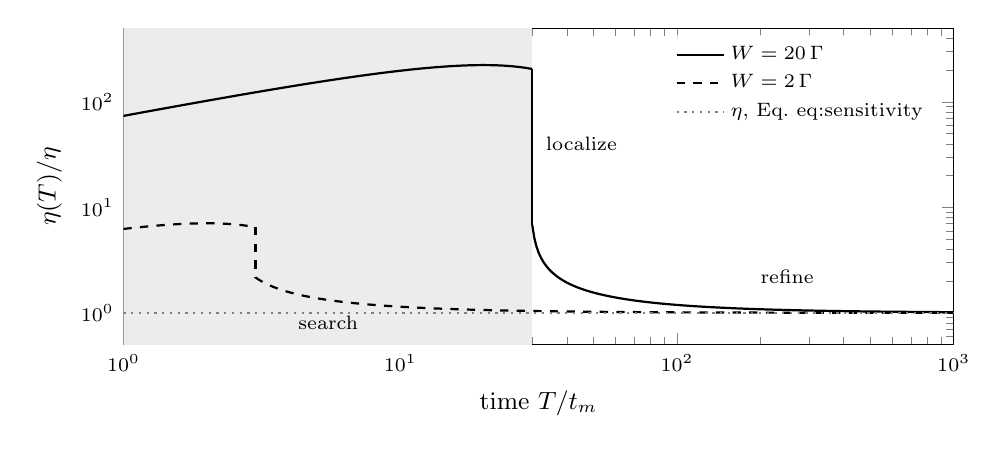
\begin{tikzpicture}
\begin{loglogaxis}[
  width=\linewidth, height=5.6cm,
  xlabel={time $T/t_m$}, ylabel={$\eta(T)/\eta$},
  xmin=1, xmax=1000, ymin=0.5, ymax=500,
  legend style={font=\scriptsize, at={(0.98,0.98)}, anchor=north east, draw=none, fill=white, fill opacity=0.8,
    text opacity=1},
  legend cell align=left,
  label style={font=\small}, tick label style={font=\scriptsize},
]
% Same illustrative values as Fig. budget: SNR = 10, k = 1, Delta x = Gamma/3 -> I* = 168.75 / Gamma^2;
% eta(T)/eta = sigma(n) sqrt(n I*), n = T/t_m.
\fill[gray!15] (axis cs:1,0.5) rectangle (axis cs:30,500);
\node[font=\scriptsize] at (axis cs:5.5,0.8) {search};
\node[font=\scriptsize, anchor=west] at (axis cs:31,40) {localize};
\node[font=\scriptsize] at (axis cs:250,2.2) {refine};
\addplot[thick, domain=1:30, samples=60] {(20 - x/3)/sqrt(12)*sqrt(168.75*x)};
\addlegendentry{$W=20\,\Gamma$}
\addplot[thick, forget plot] coordinates {(30, 205.4) (30, 6.847)};
\addplot[thick, forget plot, domain=30:1000, samples=200] {sqrt(168.75*x/(108 + 168.75*(x-30)))};
\addplot[thick, dashed, domain=1:3, samples=20] {(2 - x/3)/sqrt(12)*sqrt(168.75*x)};
\addlegendentry{$W=2\,\Gamma$}
\addplot[thick, dashed, forget plot] coordinates {(3, 6.495) (3, 2.165)};
\addplot[thick, dashed, forget plot, domain=3:1000, samples=200] {sqrt(168.75*x/(108 + 168.75*(x-3)))};
\addplot[gray, dotted, thick, domain=1:1000, samples=2] {1};
\addlegendentry{$\eta$, Eq.~\eqref{eq:sensitivity}}
\end{loglogaxis}
\end{tikzpicture}
\caption{Expected sensitivity $\eta(T)=\sigma_B(T)\sqrt T$ of an adaptive strategy as a function of the run time,
from the elimination model with the values of Fig.~\ref{fig:budget}. Solid: wide window, $W=20\,\Gamma$; dashed:
narrow window, $W=2\,\Gamma$; dotted: the refine limit $\eta$ of Eq.~\eqref{eq:sensitivity}, which is also the
unbiased Cram\'er--Rao bound. During the search (shaded) $\eta(T)$ grows as $\sqrt T$; detection drops it, and in
refine it approaches $\eta$ from above with an excess $n_e t_m/2T$, Eq.~\eqref{eq:sensitivity-time}. Simulated and
measured runs are shown against $\eta$ in Sec.~\ref{sec:results}.}
\label{fig:sensitivity-time}
\end{figure}
